
\documentclass[10pt]{article} % For LaTeX2e
% \usepackage{tmlr}
% If accepted, instead use the following line for the camera-ready submission:
% \usepackage[accepted]{tmlr}
% To de-anonymize and remove mentions to TMLR (for example for posting to preprint servers), instead use the following:
\usepackage[preprint]{tmlr}

% Optional math commands from https://github.com/goodfeli/dlbook_notation.
\input{math_commands.tex}

\usepackage{hyperref}
\usepackage{url}
\usepackage{graphicx}



\title{Formatting Instructions for TMLR \\Journal Submissions}

% Authors must not appear in the submitted version. They should be hidden
% as long as the tmlr package is used without the [accepted] or [preprint] options.
% Non-anonymous submissions will be rejected without review.

\author{\name Student number: 22033917 \\
      \addr GitHub repository: https://github.com/UCL-ELEC0136/10-final-assessment-xzzc666
      }

% The \author macro works with any number of authors. Use \AND 
% to separate the names and addresses of multiple authors.

\newcommand{\fix}{\marginpar{FIX}}
\newcommand{\new}{\marginpar{NEW}}

\def\month{01}  % Insert correct month for camera-ready version
\def\year{2026} % Insert correct year for camera-ready version


\begin{document}


\maketitle

\begin{abstract}

\end{abstract}

\section{Introduction}

\section{System overview}

\section{Data discovery and acquisition}

  \subsection{Data Sources and Usage Protocols}
    This project uses \textbf{FRED} (Federal Reserve Economic Data) as the primary data source. 
    \textbf{FRED} provides a large collection of authoritative macroeconomic and financial time--series data and supports programmatic access through a free API key.

    According to the official \textit{FRED API Terms of Use} \cite{FRED API Terms of Use}, the free API may be used for academic research and non--commercial purposes. 
    In this project, all retrieved data are used exclusively for model training and analysis. 
    The original data are neither shared nor redistributed, and the usage fully complies with the relevant terms and conditions.

    In addition, the official \textbf{FRED} website provides comprehensive API documentation\cite{FRED ALL API} to guide standardized access to economic and financial time--series data. 
    Since the data acquisition process in this project is based on indicator (series) identifiers, the \textit{series observations} endpoint in the \textbf{FRED} API documentation is primarily referenced\cite{FRED SERIES API}. 
    In the implementation, HTTP requests are sent using Python's \texttt{requests} library, with the parameters \texttt{api\_key}, \texttt{file\_type}, \texttt{series\_id}, \texttt{realtime\_start}, and \texttt{realtime\_end} used to control the type and time range of the retrieved time series. 
    This design enables an automated and fully reproducible data collection pipeline.

  \subsection{Dataset Selection}

    Table~\ref{tab:data_sources} summarises the data collected in this project and the rationale for selecting each data source. 
    Due to space limitations, the full table is reported in \textit{Appendix}. 

    In total, \textbf{31 distinct time-series datasets} are incorporated in this study. 
    These datasets are organised into multiple economically meaningful categories, including the \textit{target market}, \textit{auxiliary equity markets}, \textit{volatility and systemic risk}, \textit{credit spreads}, \textit{interest rates and term structure}, \textit{inflation}, \textit{liquidity and monetary conditions}, \textit{labour market}, \textit{economic activity}, \textit{housing market}, and \textit{consumption and sentiment}. 
    This structured design enables the model to characterise market behaviour from complementary macro-financial perspectives rather than relying on a single information source.

    The dataset spans the period from \textbf{January 1, 2015} to \textbf{December 31, 2025}, covering multiple market regimes and macroeconomic cycles.

    In the following training stage shows that using a limited number of input variables led to pronounced overfitting, particularly under high-capacity model configurations. 
    Therefore, a relatively large set of macroeconomic and financial indicators is intentionally adopted. 

    Although incorporating numerous input variables increases the dimensionality of the feature space, this challenge is addressed in later stages (\textit{Representation Learning, Feature Design, and Impact Analysis}) through Principal Component Analysis (PCA). 
    PCA enables effective dimensionality reduction while preserving the dominant information structure, thereby mitigating the negative impact of dimensionality growth on model training and generalisation performance.


  \subsection{Data storage and log writing}
  Data storage is necessary because repeatedly retrieving identical historical data through APIs not only leads to access rate limitations and increased server load, but also significantly raises the time cost of data acquisition. 
  During model training and multiple experimental runs, storing all data in a unified local database effectively avoids redundant requests, improves overall computational efficiency, and ensures data consistency as well as the reproducibility of experimental results.

  In this project, an SQLite database is adopted as the data storage solution. 
  SQLite is a lightweight local database natively supported by Python, offering advantages such as offline operation, no account configuration, and simple deployment. 
  Since the data in this project only need to be fully acquired once and stored for long-term use—without requirements for data sharing, high-concurrency access, or frequent write operations—a local database solution is sufficient to meet all project needs. 
  Furthermore, SQL is selected instead of a NoSQL database to ensure strict temporal alignment across different macroeconomic and financial indicators, thereby avoiding data mismatch issues caused by flexible or non-uniform field structures. 
  This design improves the structural stability and overall reliability of the dataset.

  \begin{figure}[t]
  \centering
  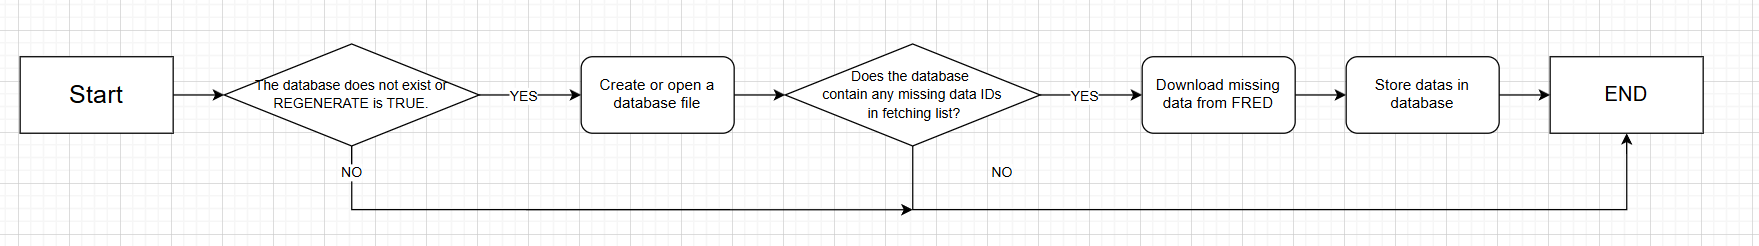
\includegraphics[width=\linewidth]{figures/data_store.png}
  \caption{Data acquisition and storage workflow}
  \label{fig:data_pipeline}
  \end{figure}


  The overall execution logic is illustrated in Figure~\ref{fig:data_pipeline}. 
  A hyperparameter \texttt{REGENERATE} is introduced to control whether the raw feature data should be regenerated. 
  When \texttt{REGENERATE} is set to \texttt{true} or when the database file does not exist, the program automatically detects missing data series and sends API requests only for the missing components. 
  The complete dataset is then stored in the \texttt{data\_raw.db} database located in the \texttt{data} directory.

  In addition, to facilitate runtime monitoring and the identification of potential errors, a \texttt{WriteLog} function is implemented. 
  This function outputs progress information and error messages to the terminal while simultaneously recording them in the \texttt{data\_fetch.log} file under the \texttt{data} directory, thereby enhancing the traceability and debugging efficiency of the data collection pipeline.


  
    


\section{Object model, data validation, and storage}
\section{Dataset construction and sampling} 
\section{Problem formalisation}
\section{Representation learning, feature design and impact analysis}
\section{Training and evaluation protocol}
\section{References}
\section{Appendix}


\begin{table}[t]
\caption{Dataset selected for model training and evaluation.}
\label{tab:data_sources}
\begin{center}
\begin{tabular}{p{3.4cm} p{4.8cm} p{6.2cm}}
\multicolumn{1}{c}{\bf CATEGORY} &
\multicolumn{1}{c}{\bf INDICATORS} &
\multicolumn{1}{c}{\bf REASON}
\\ \hline \\

Target market
& SP500
& Serves as the prediction target, providing the reference equity dynamics for supervised learning \\[6pt]

Auxiliary equity markets
& DJIA, NASDAQCOM
& Capture cross-market co-movement and sectoral divergence that may provide contextual signals for SP500 price dynamics \\[6pt]

Volatility and systemic risk
& VIXCLS, TEDRATE, STLFSI4
& Provide forward-looking information on market uncertainty, which may influence risk premia and short-term SP500 fluctuations \\[6pt]

Credit spreads
& BAMLH0A0HYM2, BAMLC0A0CM, BAMLC0A1CAAA, BAMLC0A4CBBB
& Reflect changes in financing conditions and investor risk appetite that can affect equity valuation and market drawdowns \\[6pt]

Interest rates and term structure
& GS3M, GS2, GS10, GS30, T10Y2Y, T10Y3M
& Encode monetary policy stance and yield curve expectations that influence discount rates applied to SP500 constituents \\[6pt]

Inflation
& CPIAUCSL, CPILFESL, PCEPI
& Capture inflation dynamics that shape policy expectations and indirectly impact equity valuation levels \\[6pt]

Liquidity and monetary conditions
& M2SL, WALCL
& Represent liquidity expansion or contraction that may amplify or suppress SP500 market momentum \\[6pt]

Labour market
& UNRATE, PAYEMS
& Indicate employment conditions affecting household income, consumption capacity, and earnings expectations of SP500 firms \\[6pt]

Economic activity
& INDPRO, TCU, DGORDER
& Describe real economic momentum that may influence corporate profitability and medium-term equity trends \\[6pt]

Housing market
& CSUSHPISA, HOUST, PERMIT
& Reflect interest-rate-sensitive economic sectors that often respond early to policy shifts impacting broader equity markets \\[6pt]

Consumption and sentiment
& UMCSENT, RSAFS
& Provide behavioural signals of household expectations that may affect equity demand and short-term market sentiment \\

\end{tabular}
\end{center}
\end{table}



\end{document}
